\documentclass{beamer}
\usepackage[utf8]{inputenc}
\usepackage{graphicx, epsfig}
\usepackage{amsmath,mathrsfs,amsfonts,amssymb}
\usepackage{subfig}
\usepackage{floatflt}
\usepackage{epic,ecltree}
\usepackage{mathtext}
\usepackage{fancybox}
\usepackage{fancyhdr}
\usepackage{bm}
\usepackage{multirow}
\usepackage{enumerate}
\usepackage{epstopdf}
\usepackage{multicol}
\usetheme{Copenhagen}%{Singapore}%{Warsaw}%{Warsaw}%{Darmstadt}
\usecolortheme{whale}
%\definecolor{beamer@blendedblue}{RGB}{15,120,80}

\newcommand{\T}{{\text{\tiny\sffamily\upshape\mdseries T}}}
\DeclareMathOperator*{\argmax}{arg\,max}
%--------------------------------------------------------------------------------
\title[\hbox to 56mm{Bayesian Neural Networks  \hfill\insertframenumber\,/\,\inserttotalframenumber}]
{Bayesian Neural Networks}
\author[ROY team]{\\
	{\small \textbf{ROY team:} Ilya Zharikov, \\ \hspace{2.67cm}Roman Isachenko, \\ \hspace{2.61cm}Artem Bochkarev}}
\institute[SkolTech]{Skolkovo Institute of Science and Technology \\
	Bayesian Methods course 
	\vspace{0.3cm}
}
\date{May 25, 2017}
%--------------------------------------------------------------------------------
\begin{document}
	%--------------------------------------------------------------------------------
	\begin{frame}
		%\thispagestyle{empty}
		\titlepage
	\end{frame}
%--------------------------------------------------------------------------------
\begin{frame}{Project goal}
		
	\begin{block}{Aim}
		Estimate posterior distribution of the model parameters from data
	\end{block}
	\begin{block}{Problem}
		Monte Carlo sampling is very slow for high-dimensional data
	\end{block}	
	\textbf{Probabilistic Programming}
	\begin{itemize}
		\item Uncertainty in predictions
		\item Uncertainty in representations
		\item Regularizations with priors
		\item Transfer learning
		\item Hiearchical Neural Networks
	\end{itemize}
\end{frame}
%--------------------------------------------------------------------------------
\begin{frame}{Related work}
	\begin{enumerate}
		\item Salvatier J, Wiecki T.\,V., Fonnesbeck C. Probabilistic programming in Python using PyMC3. // \emph{PeerJ Computer Science}. 2016.
		\vfill
		\item Blundell C. et al. Weight Uncertainty in Neural Network // \emph{Proceedings of The 32nd International Conference on Machine Learning}. 2015.
		\vfill
		\item Kucukelbir A. et al. Automatic Differentiation Variational Inference // \emph{arXiv preprint arXiv:1603.00788}. – 2017.
	\end{enumerate}
	
\end{frame}
%--------------------------------------------------------------------------------
\begin{frame}{Problem Statement}
	\begin{block}{Bayes Theorem}
	\[
		p(\theta|X) = \frac{p(X|\theta) p(\theta)}{p(X)}
	\]
	\end{block}
	\begin{block}{Frequentist approach}
	\[
	\theta^* = \argmax_\theta p(\theta|X) =\argmax_\theta  p(X|\theta) + p(\theta)
	\]
	\end{block}
	\textbf{Monte Carlo approach}
	\begin{itemize}
		\item Metropolis Hasting
		\item Gibbs sampling
		\item No-U-Turn Sampling (NUTS)
	\end{itemize}
\end{frame}
%--------------------------------------------------------------------------------
\begin{frame}{Variational Inference}
	\[
		\ln p(X) = \text{KL}(q||p) + \text{ELBO}(q)
	\]
	\[
		\text{KL}(q||p) = \int q(\theta) \ln \frac{q(\theta)}{p(\theta|X)} d \theta;
	\quad
		\text{ELBO}(q) = \int q(\theta) \ln \frac{p(X, \theta)}{q(\theta)}d\theta
	\]
	\begin{block}{Problem}
		minimization of $\text{KL}(q||p)$ $\Leftrightarrow$ maximization of $\text{ELBO}(q)$ 
	\end{block}
	\begin{block}{ADVI}
	\begin{itemize}
		\item Transformation of constrained variables
		\item $q(\theta)$ comes from parametric family (usually $\mathcal{N}(\mu, \text{diag}(\sigma^2))$)
		\item Stochastic optimization
		\item Integral differentiation $\Rightarrow$ reparametrization trick
	\end{itemize}
	\end{block}
\end{frame}
%--------------------------------------------------------------------------------
\begin{frame}{Neural Networks}
	\begin{itemize}
	\item \textbf{Neural networks} predict values of parameters by fitting complex model on the huge dataset
	\item \textbf{Bayesian Neural Networks} predict the parameters distributions
	\end{itemize}
	\begin{figure}
		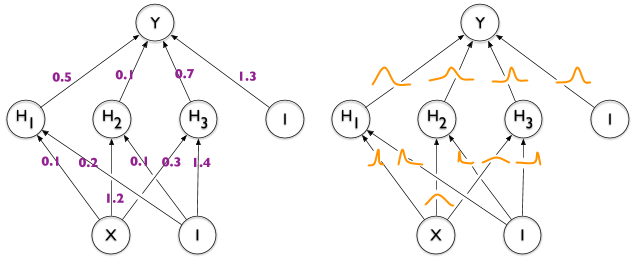
\includegraphics[width=1\linewidth]{pres_pics/BNN}
	\end{figure}
	
	\hrulefill
	
	\scriptsize{http://bit.ly/2rMQuDq}

\end{frame}
%--------------------------------------------------------------------------------

\end{document} 